\section{Tecnologie utilizzate}
Di seguito si descrivono le tecnologie e le motivazioni del loro utilizzo per la realizzazione del sito. Inoltre per ogni tecnologia si mettono in evidenza alcune meccaniche di implementazione che altrimenti potrebbero non essere ovvie guardando il codice.

\subsection{HTML 5}
La scelta di utilizzare \texttt{HTML 5} � stata motivata dal fatto che questa tecnologia � moderna ma retrocompatibile (almeno in parte). Per favorire la retrocompatibilit� non sono stati utilizzati i tag semantici introdotti da \texttt{HTML 5} (quali ad esempio, \texttt{nav, footer, section}). Infine questa tecnologia offre la possibilt� di utilizzare i \texttt{data-*attributes} i quali permettono di associare in modo semplice dati a tag (ovvero si possono memorizzare dei dati all'interno dei tag html). 

\subsection{CSS}
Per la gestione del layout del sito, il \texttt{CSS embedded} � stato evitato completamente, a favore di una separazione completa tra layout e struttura attraverso l'utlizzo di fogli di stile: lo standard adottato � il \texttt{CSS 3.0}.
\\
In fase di realizzazione del sito, si � deciso di incorporare tutti i fogli di stile in un unico file(\texttt{deafult.css}); sono stati poi realizzati layout a parte per i dispositivi mobili e per la stampa.
Sono poi presenti altri 2 fogli di stile: uno per il date-picker(vedi sezione 5.3.1) e un altro necessario per il pdf di conferma prenotazione.

\subsubsection{PDF conferma prenotazione}
I PDF generati sono creati sulla base di un template HTML sfruttando la libreria \texttt{PHP DOMPDF}. Quest'ultima permette di convertire HTML in PDF e la tipologia di tag \texttt{HTML} e attributi \texttt{CSS} a disposizione � limitata. Per gestire il layout � stato adoperato un foglio di stile a parte dedicato a tale compito.

\subsection{PHP}
\subsubsection{Dinamicit�}
PHP svolge un ruolo fondamentale per il funzionamento del sito, infatti grazie a questa tecnologia abbiamo realizzato un sito dinamico i cui contenuti (le attivit� offerte) possono essere aggiunti, modificati ed eliminati attraverso il \hyperlink{pannelloAdmin}{pannello di amministrazione}. Inoltre visto che sono presenti elementi che vengono ripetuti, come ad esempio l'intestazione e il menu, si � optato per una templetizzazione di essi e attraverso dei segnaposto nel codice \texttt{HTML} (con la seguente sintassi: [\#SEGNAPOSTO]) che vengono rimpiazzati dal contenuto attraverso \texttt{PHP}. 
Le funzioni che gestiscono operazioni come il login, la prenotazione/cancellazione di attivit�, il caricamento delle immagini e la generazione di pdf sono collocate nella cartella \texttt{php}.
Altre funzioni presenti in questa cartella sono quelle dedicate all'astrazione di elementi ricorrenti in una pagina, quali menu (desktop e mobile), pagine di errore e successo generiche.

\subsubsection{Sicurezza}
Il tema della sicurezza ha avuto un ruolo fondamentale durante la realizzazione del sito, infatti sono state create delle funzioni che permettono di garantire il controllo completo sulle operazioni che vengono richieste al server. Tale controllo consiste nel verificare quale tipologia di utente ha fatto la richiesta attraverso le informazioni contenute nella sessione; se l'utente non � un amministratore ed esso ha cercato di utilizzare delle funzionalit� riservate ad un admin allora il server rigetta la richiesta. 

\paragraph{PHP PDO - SQL Injection} \mbox{}\\
Per la connessione e l'interazione con il database � stato utilizzato \texttt{PDO} poich� permette di gestire con facilit� la connessione con diversi DBMS (nel nostro caso abbiamo utilizzato MySQL). Inoltre grazie al meccanismo di preparazione degli \texttt{statement} (statement precompilati), i dati inseriti dagli utenti vengono automaticamente sanificati in modo da impedire qualsiasi tipo di SQL Injection, questo permette l'integrit� e la sicurezza del database.
Utilizzo di metodi standard come pdo ci tutela e ci solleva dall'incombenza della manutenzione correttiva.

\subsubsection{Caricamento delle immagini}
Nel momento in cui viene creata una nuova macroattivit�, vi � la possibilit� di caricare due immagini distinte.
Tale funzionalit� � stata implementata tramite una funzione PHP \texttt{uploadImage}, che posiziona l'immagine nelle cartella\\ \texttt{images/attivita/index} e \texttt{images/attivita/banner},
una soluzione che risulta essere in linea con il principio della dinamicit� del sito gestita da PHP.


\subsection{JavaScript}
\subsubsection{Librerie}
Di seguito sono elencate le librerie JavaScript utilizzate ai fini di realizzazione del progetto.
\begin{itemize}
	\item \textbf{jquery.js}: standard de facto che semplifica la manipolazione del DOM e fornisce un'API semplice per le richieste AJAX, ampiamente utilizzate all'interno del progetto, soprattutto nella parte interna del sito.
	
	\item \textbf{jquery-asDatepicker.js:} libreria che permette di visualizzare un date-picker per la selezione di una data della prenotazione.
	
	\item \textbf{jquery-confirm.js:} Questa libreria � stata utilizzata anzitutto perch� � accessibile, infatti la finestra di dialogo viene notificata ad uno screen reader, ed � possibile iteragire con essa anche utilizzando solo la tastiera. Inoltre la libreria � semplice da utilizzare per creare finestre di dialogo  che sono state templetizzate attraverso la funzione creata da noi \\
	\texttt{generaAlert(colore,"titolo","messaggio")} che permette di creare una finestra di dialogo in modo semplice ed intuitivo. 
	
	La libreria genera finestre di dialogo pop-up di questo tipo:
	\begin{figure}[h]
		\centering
		\subfloat[][\emph{Finestra di dialogo di jquety-confirm.js}]
		{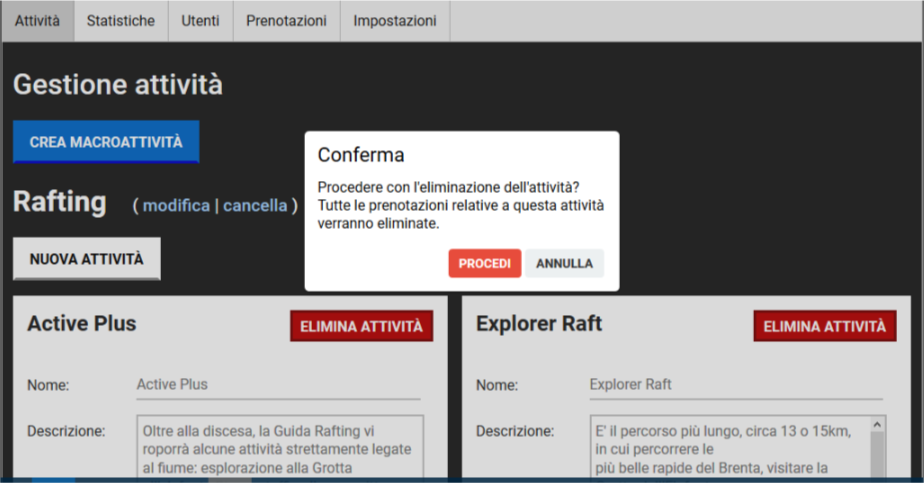
\includegraphics[scale=0.5]{images/dialog_lib.png}} 
	\end{figure}
\\
	Per le finestre di dialogo pi� complesse presenti nel pannello admin, come ad esempio quelle di inserimento di una nuova macroattivit�, si � deciso di creare dei template HTML che vengono modificati in PHP e visualizzati attraverso JS, ovviamente si ha avuto particolare riguardo per l'accessibilit� (vedi \hyperlink{aria}{Tag WAI-ARIA}).
	\begin{figure}[h]
		\centering
		\subfloat[][\emph{Finestra di dialogo creata da noi}]
		{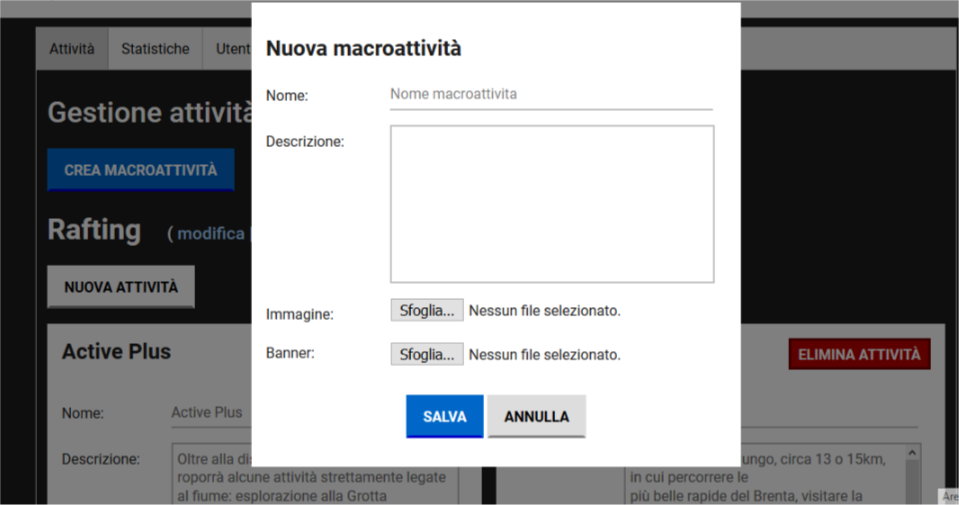
\includegraphics[scale=0.5]{images/dialog.png}} 
	\end{figure}
	
\end{itemize}

\subsubsection{JS obbligatorio}
Nelle pagine interne del sito, pannello admin e pannello utente, Javascript � richiesto affinch� sia possibile utilizzare le  funzionalit� offerte da esse. Questa scelta � stata fatta per mettere al primo posto la "fluidit'a" di utilizzo di tali pagine. Infatti, senza l'ausilio di Javascript, si incorrerebbe in innumerevoli reindirizzamenti verso pagine diverse (per quasi ogni interazione con gli elementi del pannello).\\Grazie a Javascript, invece, � possibile inserire, modificare ed eliminare elementi all'interno della pagina senza dover rirenderizzare (quindi ricaricare) l'intera pagina. Pertanto � possibile, ad esempio, mostrare finestre di dialogo e messaggi di vario tipo, inserire dinamicamente elementi in tabelle o liste e prevalidare form senza dover indirizzare l'utente verso una pagina "secondaria", che magari differisce dalla "principale" solo per un elemento in pi� visualizzato o nascosto.\\
Nel caso in cui i pannelli dovessero essere utilizzabili senza suddetta tecnologia abilitata allora viene visualizzato un messaggio di errore che avverte l'utente di abilitare Javascript per poter utilizzare le funzionalit�.
Infine, sempre nei pannelli utente ed admin, Javascript permette l'invio dei dati dei vari form tramite chiamate HTTP asincrone, senza necessit� di ricaricamento della pagina (grazie ad AJAX).
\subsubsection{AJAX}
Come detto in precedenza AJAX permette di eseguire richieste asincrone al server che vengono inoltrate a specifiche pagine PHP le quali sono adibite all'elaborazione delle richieste, come ad esempio la creazione, modifica od eliminazione di una macroattivit�
% richieste ajax
% js obbligatorio



\newpage
\subsection{Database}
Si � deciso di utilizzare MySQL (MariaDB) per la gestione del database contenente i dati del sito. 
Segue uno schema UML delle tabelle 
\begin{figure}[h]
	\centering
	\subfloat[\emph{Struttura del DB}]
	{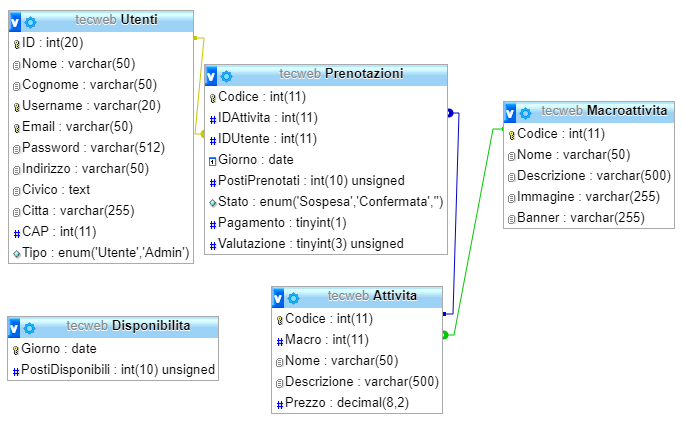
\includegraphics[scale=0.7]{images/erdb.png}}
\end{figure}
\\
Il database � privo di trigger per favorire il disaccoppiamento tra il sito e il DBMS. Si � quindi utilizzato \texttt{PHP} per le varie operazioni al fine di apprenderlo al meglio.
